\documentclass[Main.tex]{subfiles} 
\begin{document}

\section{Specifikations- og analysearbejdet}
%En uddybning af metodeafsnittet, herunder med henblik p� analysearbejdet (Domaine, Use Cases, SSD). Hvad har der v�ret af problemer undervejs, og hvorfor har vi valgt de metoder vi har valgt.
Ved p�begyndelse af projektet blev der udarbejdet en dom�nemodel, for at skabe et overblik over systemet. Denne blev dannet ud fra de informationer, der blev givet i produktopl�gget og var derfor langt fra komplet (modellen ses p� figur \ref{fig:Domain_first}). 
%\begin{figure}[H]
%\centering
%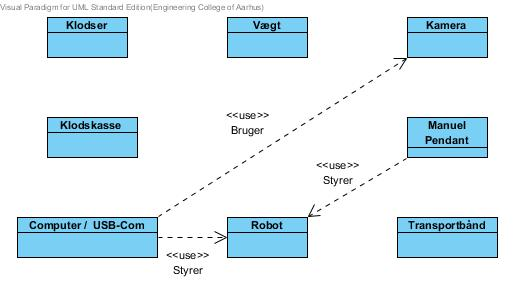
\includegraphics[scale=0.5]{../../04_Systemdesign/Diagrammer/Domain_model/Original_15_02.jpg}
%\caption{F�rste udkast af dom�nemodellen}
%\label{fig:Domain_first}
%\end{figure}
Efter tilegnelse af mere viden blev dom�nemodellen udvidet og specificeret. Der blev derudover gjort overvejelser om, hvordan de forskellige elementer interagerer med hinanden. Dette ledte til en model med den f�rste anskuelse af det system, der skulle udvikles (modellen ses p� figur \ref{fig:Domain_second}) 
%\begin{figure}[H]
%\centering
%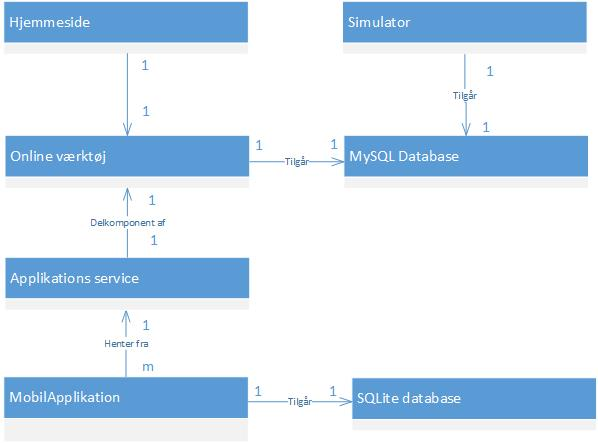
\includegraphics[scale=0.5]{../../04_Systemdesign/Diagrammer/Domain_model/Domainmodel_Billede.jpg}
%\caption{Andet udkast af dom�nemodellen}
%\label{fig:Domain_second}
%\end{figure}
Ved hj�lp af denne dom�nemodel, blev der udt�nkt brugssituationer af systemet samt overvejet, hvilke akt�rer systemet ville have. Under denne proces blev et Use Case diagram udviklet, hvilket gav et overblik over disse brugssituationer samt hvilke akt�rer, der interagerer med Use Casene (se figur \ref{fig:UseCase}).
%\begin{figure}[H]
%\centering
%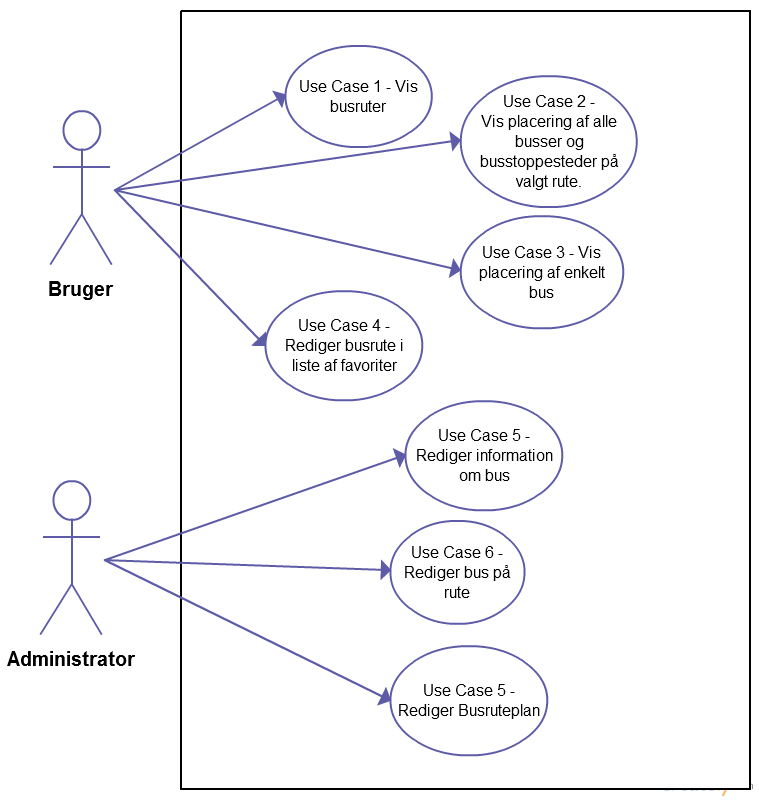
\includegraphics[scale=0.5]{../../02_Kravspecifikation/Use_Cases/Diagrammer/Use_Case_Diagram.jpg}
%\caption{Use Case diagram}
%\label{fig:UseCase}
%\end{figure}
Use Case diagrammet der ses p� ovenst�ende figur, er det endelige diagram. I takt med at systemet er blevet udviklet, er der blevet gjort erfaringer og indsamlet viden. Denne viden har gjort, at diagrammet er blevet forbedret og dermed afspejler det system, der blev udviklet.\\
Ud fra Use Casene i diagrammet, samt kravene i produktopl�gget, blev der udformet en kravspecifikationen. Her blev alle kravene til Use Casene specificeret, og disse indbefatter bl.a. scenarier af, hvorledes Use Casene opfylder de m�l, de er sat til. Denne kravspecifikationen er ligesom Use Case diagrammet s� vidt muligt blevet holdt opdateret. Dette er naturligvis gjort i samarbejde med kunden.\\
Til at bekr�fte, at kravene der blev stillet er opfyldt, blev der specificeret en accepttestspecifikation, der beskriver hvordan alle kravene skal testes. Denne er ved f�rdigg�relsen af systemet k�rt igennem sammen med kunden.\\\\
F�r udvikling p� hver del af systemet blev p�begyndt, er der blev gjort betragtninger over, hvorledes systemet snakker sammen med lag og akt�rer via simple sekvensdiagrammer. P� denne m�de er et overblik f�r udvikling blevet dannet, hvilket har hjulpet til en mere solid og problemfri udvikling. Dette er kun gjort ved de dele af systemet, hvor det er fundet fordelagtigt.
\\\\  
Generelt har analyse- og specifikationsarbejdet fungeret rigtig godt. Overblikket over dom�net og systemet har v�ret bibeholdt gennem hele projektet. Det skyldtes bl.a., at designkritiske beslutninger l�bende er blevet diskuteret af hele gruppen, hvilket medf�rte at fokus p� den rigtige funktionalitet blev bibeholdt. Det skal dog n�vnes, at der ogs� er blevet udviklet ekstra funktionaliteter, der ikke direkte er specificeret, da der ikke er fundet tid og overskud hertil.
M�den hvorp� kravene er delt op i Use Cases, har ogs� gjort det muligt at opdele opgaverne blandt gruppemedlemmerne p� en god og effektiv m�de.

\end{document}